\documentclass[10pt]{article}


% This is a helpful package that puts math inside length specifications
\usepackage{multirow}
\usepackage{wasysym}
\usepackage{marginnote}
\usepackage{url}
\usepackage{calc}
\usepackage[spanish, es-tabla]{babel}
\usepackage[utf8]{inputenc}
\usepackage{graphicx}
\usepackage{xcoffins}
\usepackage{array}
\usepackage{multicol}
\usepackage{multirow}
\usepackage{titlesec}
\usepackage[scaled=.90]{helvet}
\usepackage{fancyhdr}
\usepackage{markdown}
\usepackage[ddmmyyyy,hhmmss]{datetime}
\titleformat{\section}
  {\normalfont\sffamily\Large\bfseries\color{cyan}}
  {\thesection}{1em}{}

% Layout: Puts the section titles on left side of page
\reversemarginpar

%
%         PAPER SIZE, PAGE NUMBER, AND DOCUMENT LAYOUT NOTES:
%
% The next \usepackage line changes the layout for CV style section
% headings as marginal notes. It also sets up the paper size as either
% letter or A4. By default, letter was used. If A4 paper is desired,
% comment out the letterpaper lines and uncomment the a4paper lines.
%
% As you can see, the margin widths and section title widths can be
% easily adjusted.
%
% ALSO: Notice that the includefoot option can be commented OUT in order
% to put the PAGE NUMBER *IN* the bottom margin. This will make the
% effective text area larger.
%
% IF YOU WISH TO REMOVE THE ``of LASTPAGE'' next to each page number,
% see the note about the +LP and -LP lines below. Comment out the +LP
% and uncomment the -LP.
%
% IF YOU WISH TO REMOVE PAGE NUMBERS, be sure that the includefoot line
% is uncommented and ALSO uncomment the \pagestyle{empty} a few lines
% below.
%

%% Use these lines for letter-sized paper
\usepackage[paper=letterpaper,
            %includefoot, % Uncomment to put page number above margin
            marginparwidth=1.0in,     % Length of section titles
            marginparsep=.05in,       % Space between titles and text
            margin=1in,               % 1 inch margins
            includemp]{geometry}

%% Use these lines for A4-sized paper
%\usepackage[paper=a4paper,
%            %includefoot, % Uncomment to put page number above margin
%            marginparwidth=30.5mm,    % Length of section titles
%            marginparsep=1.5mm,       % Space between titles and text
%            margin=25mm,              % 25mm margins
%            includemp]{geometry}

%% More layout: Get rid of indenting throughout entire document
\setlength{\parindent}{0in}

%% This gives us fun enumeration environments. compactitem will be nice.
\usepackage{paralist}


%% Reference the last page in the page number
%
% NOTE: comment the +LP line and uncomment the -LP line to have page
%       numbers without the ``of ##'' last page reference)
%
% NOTE: uncomment the \pagestyle{empty} line to get rid of all page
%       numbers (make sure includefoot is commented out above)
%
\usepackage{fancyhdr,lastpage}
\pagestyle{fancy}
%\pagestyle{empty}      % Uncomment this to get rid of page numbers
\fancyhf{}\renewcommand{\headrulewidth}{0pt}
\fancyfootoffset{\marginparsep+\marginparwidth}
\newlength{\footpageshift}
\setlength{\footpageshift}
          {0.5\textwidth+0.5\marginparsep+0.5\marginparwidth-2in}
\lfoot{\hspace{\footpageshift}%
       \parbox{4in}{\, \hfill %
                    \arabic{page} / \protect\pageref*{LastPage} % +LP
%                    \arabic{page}                               % -LP
                    \hfill \,}}

% Finally, give us PDF bookmarks
\usepackage{color,hyperref}
\definecolor{darkblue}{rgb}{0.0,0.0,0.3}
\hypersetup{colorlinks,breaklinks,
            linkcolor=darkblue,urlcolor=darkblue,
            anchorcolor=darkblue,citecolor=darkblue}

%%%%%%%%%%%%%%%%%%%%%%%% End Document Setup %%%%%%%%%%%%%%%%%%%%%%%%%%%%


%%%%%%%%%%%%%%%%%%%%%%%%%%% Helper Commands %%%%%%%%%%%%%%%%%%%%%%%%%%%%

% The title (name) with a horizontal rule under it
%
% Usage: \makeheading{name}
%
% Place at top of document. It should be the first thing.
\newcommand{\makeheading}[1]%
        {\hspace*{-\marginparsep minus \marginparwidth}%
         \begin{minipage}[t]{\textwidth+\marginparwidth+\marginparsep}%
                {\large \bfseries #1}\\[-0.15\baselineskip]%
                 \rule{\columnwidth}{1pt}%
         \end{minipage}}

% The section headings
%
% Usage: \section{section name}
%
% Follow this section IMMEDIATELY with the first line of the section
% text. Do not put whitespace in between. That is, do this:
%
%       \section{My Information}
%       Here is my information.
%
% and NOT this:
%
%       \section{My Information}
%
%       Here is my information.
%
% Otherwise the top of the section header will not line up with the top
% of the section. Of course, using a single comment character (%) on
% empty lines allows for the function of the first example with the
% readability of the second example.
\renewcommand{\section}[2]%
        {\pagebreak[2]\vspace{1.3\baselineskip}%
         \phantomsection\addcontentsline{toc}{section}{#1}%
         \hspace{0in}%
         \marginpar{
         \raggedright \scshape #1}#2}

% An itemize-style list with lots of space between items
\newenvironment{outerlist}[1][\enskip\textbullet]%
        {\begin{itemize}[#1]}{\end{itemize}%
         \vspace{-.6\baselineskip}}

% An environment IDENTICAL to outerlist that has better pre-list spacing
% when used as the first thing in a \section 
\newenvironment{lonelist}[1][\enskip\textbullet]%
        {\vspace{-\baselineskip}\begin{list}{#1}{%
        \setlength{\partopsep}{0pt}%
        \setlength{\topsep}{0pt}}}
        {\end{list}\vspace{-.6\baselineskip}}

% An itemize-style list with little space between items
\newenvironment{innerlist}[1][\enskip\textbullet]%
        {\begin{compactitem}[#1]}{\end{compactitem}}

% To add some paragraph space between lines.
% This also tells LaTeX to preferably break a page on one of these gaps
% if there is a needed pagebreak nearby.
\newcommand{\blankline}{\quad\pagebreak[2]}

%%%%%%%%%%%%%%%%%%%%%%%% End Helper Commands %%%%%%%%%%%%%%%%%%%%%%%%%%%

%%%%%%%%%%%%%%%%%%%%%%%%% Begin CV Document %%%%%%%%%%%%%%%%%%%%%%%%%%%%

\newcolumntype{M}[1]{>{\centering\arraybackslash}m{#1}}
\newcolumntype{P}[1]{>{\hfill\arraybackslash}p{#1}}

\begin{document}
%{\sffamily 
%\marginnote{typeset text here...}
%{\fontfamily{cmss}\selectfont

\makeheading{\begin{tabular}{l P{40mm}}
  &  \textit{\footnotesize{Updated:}}   \\
PhD Rodrigo López Farías. \footnotesize{\textit{Computer Science and Engineering}  } & \footnotesize{\textit{\today}}
\end{tabular}
}




\section{Personal Information} 
\begin{tabular}{l P{54mm} M{5mm}}
Birthday: 8-Jul-1984		&	e-mail:  rdglpz@gmail.com	& \multirow{2}{*}[0.5cm]{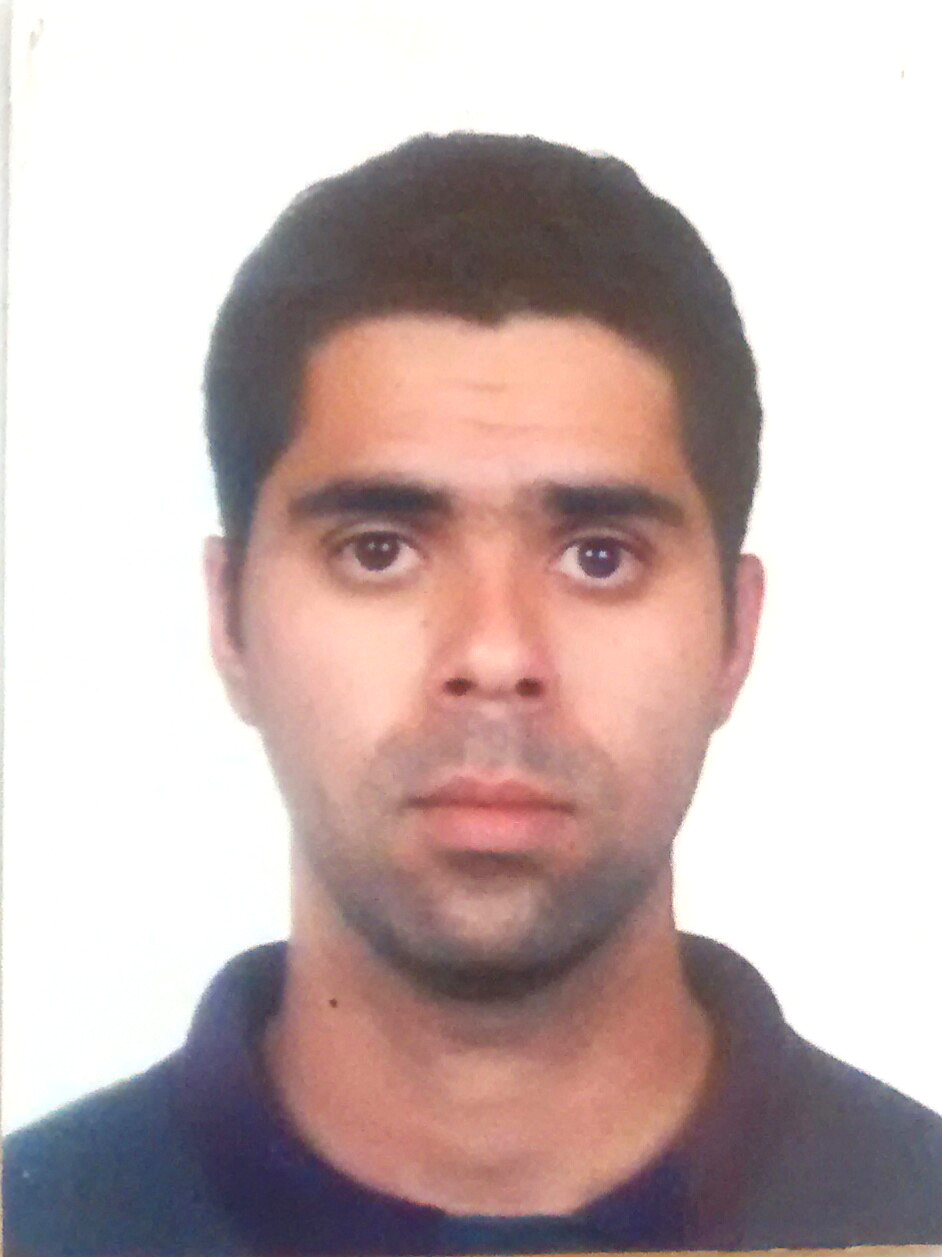
\includegraphics[width=2.0cm]{foto2.jpg}  } 	\\
Address: Membrillo \# 306, Int 3		&  Cellular: +52 443 155 5416	 		&	\\
ZIP Code: 02820		& 	Skype ID: rdglpz  			&	\\
Mexico City        		&	ORCID ID: 0000-0003-2772-0051						&
\end{tabular}

\blankline

\section{Current Job}
\textbf{Management and Coordination of Information  and Communication Technology. (CGSTIC) at the Center of Research and Advanced Studies of the Polytechnic National Institute (CINVESTAV-IPN)
%Coordinación y Gestión de Servicios de Tecnologías de Información y Comunicaciones (CGSTIC) del Centro de Investigación y Estudios Avanzados del Instituto Politécnico Nacional (CINVESTAV-IPN)}. \textit{(Oct/2016 - Actualidad)
}.
%Ciudad de Mexico, Mexico
Mexico City, Mexico

Innovation with conversational agents with Big Data

%Agentes conversacionales inteligentes manejando gran volumen de información (Big Data).

\blankline

\section{Interests \& Skills  } \textbf{Programming and Data Base Managing Languages, } 
MATLAB, MATHEMATICA, Python, R, Java, C/C++, PHP-HTML-MySQL(SQL), CassandraDB(NoSQL, Cassandra Query Language).

%ATLAB, MATHEMATICA, R, Java, C/C++, PHP-HTML-MySQL, Python, LISP.

\blankline

\textbf{Research} 

%Aprendizaje automático (Máquinas de Vectores de Soporte, Redes Neuronales Artificiales, Lógica difusa), minería de datos (Algoritmos eficientes de búsqueda de vecinos cercanos), modelado y predicción de series de tiempo, predicción multimodelo con selección probabilista de modelos (Enfoque Bayesiano).
%Optimización global no convexa con computación evolutiva, análisis de estabilidad e identificación de parámetros de sistemas dinámicos no lineales.

Modelling and time series forecasting of non-linear and/or chaotic time series applied to drinking water demand, speed wind forecasting using Machine Learning (SVM, Artificial Neural Networks, Fuzzy Logic, Nearest Neighbors). Data mining (efficient algorithms for nearest neighbors search). Probabilistic Multi-model forecasting (Bayesian Approach). Global Optimization with Evolutionary Computing, stability analysis and parameter Identification of non-linear dynamical systems. %Dimensionality reduction, time series, nonlinear dynamical systems, global optimization, evolutionary computing.
 
\blankline

\textbf{Research groups and projects}

Mexican Center of Energy Innovation Project: Forecasting the Natural Resources Required for the Production of Renewable Electric Power. \url{https://www.ineel.mx/}.

Applied Computational Intelligence Network. \url{https://goo.gl/7B4RcE}.


\blankline
 
\textbf{Languages} 

English: 550 ITP TOEFL points. 

Italyn: B1 Common CEFRL Level. 


\section{Academic Degree}  \textbf{Ph.D in Computer Science and Engineering}. (With European Doctorate mention).

IMT School of Advanced Studies Lucca. Lucca, Italy. \textit{(Feb-2012 Jan-2016)}. 

Thesis: Time Series Forecasting Based on Classification of Dynamic Patterns.

Advisors: PhD. Alberto Bemporad. PhD. Pantelis Sopasakis.

Field of study: Time series analysis.

\textbf{Taken Courses:} Semantics and Formal Methods. Complexity of Algorithms, Basic Linear Algebra. Principles of Parallel and Concurrent computing. Perfocmance Modelling applied to Computer Networks. Specification, modelling and verification of reactive systems. Global and Local Optimization Introduction. Model checking, Optimum control,  (Optimization Algorithms). Programming Methodologies, \textit{Cloud Computing}. Theory of complex networks. Machine Learning). 

\blankline

\textbf{MSc in Electrical Engineering (Computer Systems Group)}.

Universidad Michoacana de San Nicolas de Hidalgo. Morelia, Mexico. \textit{(Mar-2008 Aug-2010)}.

Thesis: Bifurcation Diagrams for Discontinuous or Non-differentiable Equations.

Advisors:  PhD. Juan Jose Flores Romero, PhD. Claudio Fuerte E.

Field of study:  Evolutionary computing, nonlinear dynamical systems, stability analysis and optimization.

\blankline

\textbf{B.Eng. in Computer Systems}.

%Instituto Tecnológico de Morelia. Morelia, Mexico. \textit{(2002 2007)}.
Morelia Institute Of Technology. Morelia, Mexico. \textit{(2002 2007)}.


Thesis: Implementation and performance analysis of \textbf{``Linux Terminal Server Project"} for educational purposes.

Field of Study: Applications of distributed operative systems.

\section{Academic Experience}  \textbf{Teaching}.


\blankline
\textbf{Morelia Institute of Technology}. Morelia, Mexico.

\begin{innerlist}
\item Structured programming and object oriented programming (Electronic and  Industrial Engineering), Research Methodology (Computational Systems Engineering). \textit{(Aug-2011 Jan-2012)}.
\item Database Fundamentals (Computational Systems Engineering), Structures and organization of data. (Technology Information Engineering) and Evaluation of software projects. \textit{(Jan-2011 Jul-2011)}.
\item Operative systems, selected topics in programming and research fundamentals. \textit{(Aug-2010 Dec-2010)}.
\end{innerlist}


\blankline

\blankline
\textbf{University of Morelia}. Morelia, Mexico.

\begin{innerlist}
\item Web programming with PHP. \textit{(Aug-2009 Dec-2009)}.
\end{innerlist}

\blankline

\section{Professional Experience}
%\subsection{Participation in Research Projects}
\textbf{State Center for Information and Communications Technologies (CETIC)}. \textit{(Mar-2007 Jun-2007)}.
Morelia, Mexico.

Resident in physical infrastructure department.

Project: Performance analysis of \textbf{Linux Terminal Server Project} applied to to basic education.

\blankline

{\textbf{Morelia Institute of Technology}}. Morelia, Mexico. \textit{(Feb-2007)}

Social Service Project: Develop of a PHP Web catalog for Social Service.

\blankline

%\textbf{IMPULSA}
%\blankline

%Participation in the young entrepreneurs program: IMPULSA.


%\blankline

\section{Publications} \textbf{Articles in Journal Citation Reports}

\blankline


\textbf{Accepted}

%\subsection{Journal Articles Sent}
\begin{innerlist}
\item \textit{Hector Rodriguez Rangel, Vicen\c{c} Puig, Rodrigo López Farías, Juan J. Flores }.  Short-Term Demand Forecast using Bank of Neural Network Models Trained using Genetic Algorithms for the Optimal Management of Drinking Water Networks.  \textit{Journal of Hydroinformatics}. DOI: 10.2166/hydro.2016.199. ISSN: 1464-7141 \textbf{November 2016}.
%\item \textit{Juan J. Flores, Rodrigo López Farías, July Barrera, Carlos Coello }.  Performance of Gravitational Interaction Optimization Metaheuristics on High Dimensional Problems.  \textit{Journal of Metaheuristics}.(2016)
%\item \textit{Juan J. Flores, José Cede\~no Gonzalez, Rodrigo López Farías, Félix Calderón }.  Evolving Nearest Neighbor Time Series Forecasters. \textit{Journal of Time Series Analysis}.(2016)
\end{innerlist}


\textbf{Under Review}
\begin{innerlist}
\item \textit{Juan J. Flores, José Cede\~no Gonzalez, Rodrigo López Farías, Félix Calderón }.  Evolving Nearest Neighbor Time Series Forecasters. (Enviado a \textit{Journal of Soft Computing, \url{https://goo.gl/hSV5SV}}, el 25 de Agosto 2016).
%\item \textit{Juan J. Flores, Rodrigo López Farías, July Barrera, Carlos Coello }.  Performance of Gravitational Interaction Optimization Metaheuristics on High Dimensional Problems.  Enviado a  \textit{Journal of Metaheuristics, \url{https://goo.gl/6bZ4tE}, el 1 de Febrero 2017}.
\end{innerlist}



\textbf{Next Submissions}
\begin{innerlist}
\item \textit{Rodrigo Lopez Farías, Vicen\c{c} Puig, Hector Rodriguez Rangel, Juan J. Flores Romero}.  Probabilistic Selection of Qualitative Prediction Models of Water Demand Time-Series (Revista tentativa: Journal of Hydroinformatics, \url{http://jh.iwaponline.com/}).
%\item \textit{Juan J. Flores, Rodrigo López Farías, July Barrera, Carlos Coello }.  Performance of Gravitational Interaction Optimization Metaheuristics on High Dimensional Problems.  Enviado a  \textit{Journal of Metaheuristics, \url{https://goo.gl/6bZ4tE}, el 1 de Febrero 2017}.
\end{innerlist}

\blankline



\textbf{Peer Reviewed Accepted Articles in National and International Conferences}

\blankline
\textbf{Accepted}
\begin{innerlist}


\item \textbf{Comparison of Time Series Forecasting Techniques with respect to Tolerance to Noise.} \textit{Juan J. Flores, Felix Calderon Solorio, Jose Rafael Cede\~no Gonzalez, Jose Ortiz Bejar and Rodrigo Lopez Farias}. (Pendiente) .\textit{IEEE Autumn Meeting on Power, Electronics and Computing}, \textbf{Ixtapa , November 2016}.


\item \textbf{Holt-Winters Residual Modelling using an ANN trained by GA and Time Series Validation Applied to Water Demand Forecasting} \textit{Hector Rodriguez-Rangel, Vicen\c{c} Puig, Juan J. Flores and ,  Rodrigo López} Farías.. (Pending). \textbf{3rd International Conference on Control and Fault-Tolerant Systems} \textbf{Barcelona, Spain. Septiembre 2016}.

\item \textbf{Flow meter Data Validation and Reconstruction using Neural Networks: Application to the Barcelona Water Network} \textit{Hector Rodriguez Rangel, Vicen\c{c} Puig,Juan J. Flores and ,  Rodrigo López Farías.}. \url{https://goo.gl/i7muz7}. \textbf{2016 European Control Conference, Aalborg. June 2016}.

\item \textbf{Qualitative and Quantitative Mul} \textit{Rodrigo López Farías, Juan J. Flores and Vicen\c{c} Puig}.  ti-Model Forecasting with Nonlinear Noise Filter Applied to Water Demand \textit{IEEE Autumn Meeting on Power, Electronics and Computing}. DOI: 10.1109/ROPEC.2015.7395122.  \textbf{Ixtapa Mexico, November 2015}.

\item \textbf{FNN a Fuzzy Version of the Nearest Neighbour Time Series Forecasting Technique } \textit{Juan J. Flores, Jose Ortiz Bejar, Jose Rafael Cedeño, Carlos Lara-Alvarez and Rodrigo López Farías}. \textit{IEEE Autumn Meeting on Power, Electronics and Computing}. DOI: 10.1109/ROPEC.2015.7395125. \textbf{Ixtapa Mexico, November 2015 }.

\item \textbf{A Multiple-Model Predictor Approach Based on an On-Line Mode Recognition with Application to Water Demand Forecasting} \textit{Rodrigo López Farías, Vicen\c{c} Puig}.  \textit{International work-conference on Time Series 1. 
} URI https://goo.gl/njWQ1e. \textbf{Granada Spain, July 2015}.

\item \textbf{An implementation of a multi-model predictor based on the qualitative and quantitative decomposition of the time-series.} \textit{Rodrigo. López, Vicen\c{c} Puig, Hector Rodriguez.} URI http: //hdl.handle.net/2117/81862. \textit{International work-conference on Time Series 1 
} \textbf{Granada Spain, July 2015}.

\item \textbf{Optimization with gravitational Interactions} \textit{Dr, Juan Flores, Rodrigo López, Julio Barrera.}   \textit{ROPEC XIII: Autumn Meeting of Electric power systems, electronic and computation ( Reunión de Oto\~no de Potencia, Electronica y Computacion)} \textbf{ Morelia Mexico, November 2011}.

\item \textbf{Gravitational Interactions Optimization.} Juan Flores, Rodrigo Lopez, Julio Barrera.  \textit{Learning and Intelligent OptimizatioN}  (LION 5) DOI 10.1007/978-3-642-25566-3\_17. \textbf{Rome, Italy - Enero 2011}. 

\item \textbf{Particle swarm optimization with gravitational interactions for multimodal and unimodal problems.} Juan J. Flores, Rodrigo Lopez and July Barrera.  In \textit{Proceedings of the 9th Mexican International Conference on Artificial Intelligence (MICAI 2010)}, pages 3361-370. Springer-Verlag. DOI 10.1007/978-3-642-16773-7\_31. \textbf{Pachuca, Mexico. November 2010.}

\end{innerlist}

\section{Conferences, Seminars \& Workshops } \textbf{Given} \begin{innerlist}
 %\item Learning and Intelligent OptimizatioN - 'Gravitational Interactions Optimization'. (Rome, Italy. Enero 2011)
\item IV National Seminar of computer learning and intelligence (SNAIC). Water demand prediction with Genetic Algorithms for the optimum optimization of a Drinking Water Distribution System. National Institute of Optics And Astrophysics (Instituto Nacional de Astrofísica, Óptica y Electrónica). Michoacan University of San Nicolas de Hidalgo (Universidad Michoacana de San Nicolás de Hidalgo). (Morelia, Mexico. September 2016).
\item 11$^o$ Congreso Estatal de Ciencia, Tecnología e Innovación, en  Ciencias de la Ingeniería y Tecnología. Búqueda del Clique con la mayor Interconectividad en un Grafo utilizando Optimización basado en Colonia de Hormigas. \textbf{Morelia, Mexico. Octubre 2016}.

%\item IV Seminario Nacional de Aprendizaje e Inteligencia Computacional (SNAIC). Predicción de la demanda de Agua con Algoritmos Genéticos para la optimización de la distribución de la Demanda de Agua en Redes de Agua Potable. Instituto Nacional de Astrofísica, Óptica y Electrónica. Universidad Michoacana de San Nicolás de Hidalgo. \textbf{Morelia, Mexico. Septiembre 2016}..



\item 11$^{th}$ State Congress of Science Technology and Innovation in  Engineering and computer Science. PSO with Interactive Niches and Quasi-Newton Local Searches. Search the most connected Clique in a Weighted Graph with Ant Colony Optimization. \textbf{Morelia, México. October 2016}.


 \item 10$^{th}$ State Congress of Science Technology and Innovation in  Engineering and computer Science. PSO with Interactive Niches and Quasi-Newton Local Searches. \textbf{Morelia, Mexico. September 2015}.


\item Activities of X Anniversary of the Instituto Tecnológico Superior de Ciudad Hidalgo - ' Evolutionary computing applied to dynamical systems'.(Ciudad Hidalgo, Mexico. October 2010).
  %\item Activities of X Anniversary of the Instituto Tecnológico Superior de Ciudad Hidalgo - ' Evolutionary computing applied to dynamical systems'.(Ciudad Hidalgo, México. October 2010).
%\item Week of Research Projects FIE of the UMSNH - 'Gravitational Interactions Optimization ' ( Morelia, Mexico. June 2010 ).
\item Week of Research Projects FIE of the UMSNH - 'Gravitational Interactions Optimization ' ( Morelia, México. Junio 2010 )
%\item Semana de Proyectos de Investigación de la Facultad de la UMSNH- 'Optimización con Interacciones Gravitacionales' \textbf{Morelia, Mexico. June 2010}.

\item Week of Research Projects FIE of the Michoacan University of San Nicolás de Hidalgo - - 'Bifurcation Diagrams using Artificial Intelligence Algorithms (Diagramas de Bifurcación Utilizando Herramientas de Inteligencia Artificia)' \textbf{Morelia, Mexico. June 2009}.
%\item Semana de Proyectos de Investigación de la Facultad de la UMSNH - 'Diagramas de Bifurcación Utilizando Herramientas de Inteligencia Artificial' \textbf{Morelia, Mexico. June 2009}.

\end{innerlist}

\blankline


\textbf{Attended}
\begin{innerlist}
\item 5th HYCON2 Ph.D. School on Control of Networked and Large-Scale Systems and the EFFINET Ph.D. School on Control of Drinking Water Networks  (Lucca Italy, 1-5 of July 2013)
\item Java workshop in the 2nd Week of Computation and Systems. \textit{Morelia, Mexico (2006).}
\item Analysis and Object Oriented Design using UML  (Morelia Mexico,  8-12 of August 2011)

%\item Taller de Java en la 2da Semana de Sistemas y Computación (Morelia Mexico, 2006)
%\item Week of Systems and computation in the Instituto Tecnológico de Morelia. \textit{Morelia, Mexico (2006)}.
%\item 2da. Semana de Sistemas y Computaci\'on en el Instituto Tecnológico de Morelia (Morelia Mexico, 2006).	
%\item Week of Systems and computation in the Instituto Tecnológico de Morelia. \textit{Morelia, Mexico (2005).}
\end{innerlist}
%}
\end{document}




%%%%%%%%%%%%%%%%%%%%%%%%%% End CV Document %%%%%%%%%%%%%%%%%%%%%%%%%%%%%

%%%%%%%%%%%%%%%%%%%%%%%%%% Git Instructions %%%%%%%%%%%%%%%%%%%%%%%%%%%%
%cd /Users/rodrigolopez/rdglpzCV/rdglpzEngCV
%git add rdglpzCVEng.tex
%git add rdglpzCVEng.pdf
%git commit -m "Changes"
%git push origin master
%%%%%%%%%%%%%%%%%%%%%%%%%%%%%%%%%%%%%%%%%%%%%%%%%%%%%%%%%%%%%%%%%%%%%%%%%


